
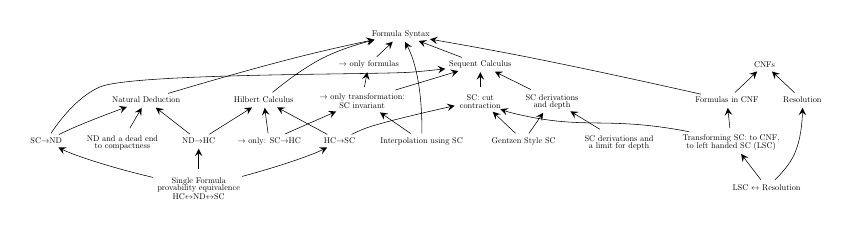
\begin{tikzpicture}[>=latex,line join=bevel,scale=0.15, every node/.style={scale=0.3}]
  \pgfsetlinewidth{1bp}
%%
\pgfsetcolor{black}
  % Edge: ND -> Formulas
  \draw [->,-stealth,very thin] (347.07bp,268.93bp) .. controls (418.11bp,290.17bp) and (548.78bp,328.42bp)  .. (661.45bp,356.9bp) .. controls (718.33bp,371.28bp) and (783.18bp,385.64bp)  .. (841.51bp,398.07bp);
  % Edge: MiniSC_HC -> MiniSC
  \draw [->,-stealth,very thin] (627.78bp,171.68bp) .. controls (658.89bp,185.38bp) and (703.61bp,205.08bp)  .. (750.65bp,225.8bp);
  % Edge: SC_Depth_Limit -> SC_Depth
  \draw [->,-stealth,very thin] (1383.3bp,182.94bp) .. controls (1363.9bp,194.79bp) and (1341.2bp,208.65bp)  .. (1312.4bp,226.22bp);
  % Edge: SCND -> ND
  \draw [->,-stealth,very thin] (84.793bp,170.22bp) .. controls (95.352bp,175.41bp) and (107.34bp,181.1bp)  .. (118.45bp,185.91bp) .. controls (158.09bp,203.06bp) and (203.67bp,220.38bp)  .. (248.05bp,236.6bp);
  % Edge: MiniSC_HC -> HC
  \draw [->,-stealth,very thin] (587.0bp,173.27bp) .. controls (585.1bp,187.68bp) and (582.41bp,207.94bp)  .. (578.88bp,234.63bp);
  % Edge: SC_Gentzen -> SC_Cut
  \draw [->,-stealth,very thin] (1180.9bp,173.27bp) .. controls (1167.6bp,185.78bp) and (1149.7bp,202.71bp)  .. (1126.2bp,224.96bp);
  % Edge: MiniSC -> MiniFormulas
  \draw [->,-stealth,very thin] (818.31bp,284.37bp) .. controls (819.89bp,292.81bp) and (821.59bp,301.9bp)  .. (825.0bp,320.1bp);
  % Edge: LSC_Resolution -> Resolution
  \draw [->,-stealth,very thin] (1803.9bp,62.046bp) .. controls (1819.4bp,77.001bp) and (1839.6bp,99.58bp)  .. (1850.4bp,123.68bp) .. controls (1865.0bp,156.07bp) and (1868.9bp,197.18bp)  .. (1869.8bp,234.58bp);
  % Edge: CNF_Formulas -> CNF
  \draw [->,-stealth,very thin] (1707.5bp,271.15bp) .. controls (1720.9bp,283.81bp) and (1738.8bp,300.83bp)  .. (1760.9bp,321.86bp);
  % Edge: NDHC -> HC
  \draw [->,-stealth,very thin] (446.21bp,171.01bp) .. controls (471.77bp,187.11bp) and (511.2bp,211.94bp)  .. (548.54bp,235.45bp);
  % Edge: SCND -> SC
  \draw [->,-stealth,very thin] (65.886bp,173.15bp) .. controls (85.526bp,202.77bp) and (128.78bp,260.21bp)  .. (182.45bp,284.13bp) .. controls (258.65bp,318.1bp) and (849.28bp,313.48bp)  .. (932.45bp,320.13bp) .. controls (955.21bp,321.95bp) and (979.7bp,324.42bp)  .. (1012.7bp,328.09bp);
  % Edge: LSC -> SC_Cut
  \draw [->,-stealth,very thin] (1597.7bp,176.96bp) .. controls (1580.7bp,180.27bp) and (1563.1bp,183.41bp)  .. (1546.4bp,185.91bp) .. controls (1381.7bp,210.64bp) and (1335.2bp,182.3bp)  .. (1173.4bp,221.91bp) .. controls (1167.2bp,223.44bp) and (1160.8bp,225.38bp)  .. (1144.6bp,231.1bp);
  % Edge: MiniSC_Craig -> MiniSC
  \draw [->,-stealth,very thin] (929.22bp,172.81bp) .. controls (910.92bp,185.38bp) and (885.89bp,202.57bp)  .. (855.35bp,223.55bp);
  % Edge: SC_Depth -> SC
  \draw [->,-stealth,very thin] (1217.8bp,278.21bp) .. controls (1193.2bp,290.43bp) and (1163.9bp,304.96bp)  .. (1131.2bp,321.22bp);
  % Edge: MiniFormulas -> Formulas
  \draw [->,-stealth,very thin] (847.88bp,356.88bp) .. controls (857.25bp,365.74bp) and (868.64bp,376.5bp)  .. (886.29bp,393.18bp);
  % Edge: LSC -> CNF_Formulas
  \draw [->,-stealth,very thin] (1695.3bp,186.14bp) .. controls (1694.0bp,198.48bp) and (1692.6bp,212.54bp)  .. (1690.3bp,234.53bp);
  % Edge: SC_Cut -> SC
  \draw [->,-stealth,very thin] (1096.4bp,284.37bp) .. controls (1096.4bp,292.72bp) and (1096.4bp,301.7bp)  .. (1096.4bp,320.1bp);
  % Edge: SC -> Formulas
  \draw [->,-stealth,very thin] (1052.6bp,355.21bp) .. controls (1024.4bp,365.96bp) and (987.56bp,380.0bp)  .. (948.4bp,394.92bp);
  % Edge: HCSC -> SC_Cut
  \draw [->,-stealth,very thin] (787.51bp,170.54bp) .. controls (798.27bp,175.93bp) and (810.71bp,181.67bp)  .. (822.45bp,185.91bp) .. controls (859.27bp,199.2bp) and (956.98bp,222.07bp)  .. (1035.0bp,239.56bp);
  % Edge: HCSCND -> SCND
  \draw [->,-stealth,very thin] (311.24bp,67.3bp) .. controls (253.14bp,81.127bp) and (180.98bp,100.47bp)  .. (118.45bp,123.68bp) .. controls (109.95bp,126.84bp) and (101.06bp,130.74bp)  .. (83.557bp,139.16bp);
  % Edge: HCSCND -> HCSC
  \draw [->,-stealth,very thin] (524.61bp,69.739bp) .. controls (576.36bp,83.725bp) and (639.43bp,102.47bp)  .. (694.45bp,123.68bp) .. controls (702.82bp,126.91bp) and (711.6bp,130.81bp)  .. (728.96bp,139.17bp);
  % Edge: MiniSC_Craig -> Formulas
  \draw [->,-stealth,very thin] (956.06bp,173.24bp) .. controls (956.68bp,209.53bp) and (955.21bp,292.28bp)  .. (932.45bp,356.9bp) .. controls (929.29bp,365.86bp) and (925.01bp,375.25bp)  .. (916.12bp,392.65bp);
  % Edge: NDHC -> ND
  \draw [->,-stealth,very thin] (398.79bp,171.68bp) .. controls (378.61bp,187.41bp) and (348.3bp,211.04bp)  .. (317.53bp,235.03bp);
  % Edge: SC_Gentzen -> SC_Depth
  \draw [->,-stealth,very thin] (1213.2bp,173.27bp) .. controls (1221.2bp,184.77bp) and (1231.8bp,200.02bp)  .. (1247.4bp,222.66bp);
  % Edge: Resolution -> CNF
  \draw [->,-stealth,very thin] (1850.6bp,270.73bp) .. controls (1837.0bp,283.48bp) and (1818.6bp,300.81bp)  .. (1796.3bp,321.7bp);
  % Edge: HCSC -> HC
  \draw [->,-stealth,very thin] (729.21bp,170.58bp) .. controls (699.08bp,186.83bp) and (651.86bp,212.32bp)  .. (608.68bp,235.62bp);
  % Edge: ND_FiniteAssms -> ND
  \draw [->,-stealth,very thin] (255.33bp,185.6bp) .. controls (262.77bp,198.43bp) and (271.33bp,213.19bp)  .. (283.77bp,234.62bp);
  % Edge: LSC_Resolution -> LSC
  \draw [->,-stealth,very thin] (1769.4bp,62.162bp) .. controls (1758.3bp,76.681bp) and (1742.4bp,97.482bp)  .. (1722.2bp,123.85bp);
  % Edge: HCSCND -> NDHC
  \draw [->,-stealth,very thin] (420.45bp,87.692bp) .. controls (420.45bp,100.68bp) and (420.45bp,114.55bp)  .. (420.45bp,136.39bp);
  % Edge: MiniSC -> SC
  \draw [->,-stealth,very thin] (892.69bp,277.18bp) .. controls (937.49bp,290.66bp) and (992.47bp,307.21bp)  .. (1043.7bp,322.65bp);
  % Edge: CNF_Formulas -> Formulas
  \draw [->,-stealth,very thin] (1625.8bp,267.22bp) .. controls (1534.0bp,287.88bp) and (1357.4bp,327.01bp)  .. (1206.4bp,356.9bp) .. controls (1131.7bp,371.71bp) and (1046.2bp,387.0bp)  .. (975.52bp,399.31bp);
  % Edge: HC -> Formulas
  \draw [->,-stealth,very thin] (597.62bp,271.22bp) .. controls (625.18bp,294.08bp) and (675.59bp,333.18bp)  .. (724.45bp,356.9bp) .. controls (758.7bp,373.53bp) and (799.09bp,386.26bp)  .. (842.86bp,397.74bp);
  % Node: HCSC
\begin{scope}
  \definecolor{strokecol}{rgb}{0.0,0.0,0.0};
  \pgfsetstrokecolor{strokecol}
  \draw (758.45bp,154.79bp) node {HC$\rightarrow$SC};
\end{scope}
  % Node: HCSCND
\begin{scope}
  \definecolor{strokecol}{rgb}{0.0,0.0,0.0};
  \pgfsetstrokecolor{strokecol}
  \draw (420.45bp,58.04bp) node {Single Formula};
  \draw (420.45bp,40.04bp) node {provability equivalence};
  \draw (420.45bp,22.04bp) node {HC$\leftrightarrow$ND$\leftrightarrow$SC};
\end{scope}
  % Node: SC_Gentzen
\begin{scope}
  \definecolor{strokecol}{rgb}{0.0,0.0,0.0};
  \pgfsetstrokecolor{strokecol}
  \draw (1200.4bp,154.79bp) node {Gentzen Style SC};
\end{scope}
  % Node: HC
\begin{scope}
  \definecolor{strokecol}{rgb}{0.0,0.0,0.0};
  \pgfsetstrokecolor{strokecol}
  \draw (576.45bp,253.02bp) node {Hilbert Calculus};
\end{scope}
  % Node: LSC_Resolution
\begin{scope}
  \definecolor{strokecol}{rgb}{0.0,0.0,0.0};
  \pgfsetstrokecolor{strokecol}
  \draw (1783.4bp,43.841bp) node {LSC $\leftrightarrow$ Resolution};
\end{scope}
  % Node: SCND
\begin{scope}
  \definecolor{strokecol}{rgb}{0.0,0.0,0.0};
  \pgfsetstrokecolor{strokecol}
  \draw (54.447bp,154.79bp) node {SC$\rightarrow$ND};
\end{scope}
  % Node: Formulas
\begin{scope}
  \definecolor{strokecol}{rgb}{0.0,0.0,0.0};
  \pgfsetstrokecolor{strokecol}
  \draw (905.45bp,411.29bp) node {Formula Syntax};
\end{scope}
  % Node: LSC
\begin{scope}
  \definecolor{strokecol}{rgb}{0.0,0.0,0.0};
  \pgfsetstrokecolor{strokecol}
  \draw (1698.45bp,159.99bp) node {Transforming SC: to CNF,};
  \draw (1698.45bp,141.99bp) node {to left handed SC (LSC)};
\end{scope}
  % Node: ND
\begin{scope}
  \definecolor{strokecol}{rgb}{0.0,0.0,0.0};
  \pgfsetstrokecolor{strokecol}
  \draw (294.45bp,253.02bp) node {Natural Deduction};
\end{scope}
  % Node: MiniFormulas
\begin{scope}
  \definecolor{strokecol}{rgb}{0.0,0.0,0.0};
  \pgfsetstrokecolor{strokecol}
  \draw (828.45bp,338.52bp) node {$\rightarrow$ only formulas};
\end{scope}
  % Node: MiniSC_HC
\begin{scope}
  \definecolor{strokecol}{rgb}{0.0,0.0,0.0};
  \pgfsetstrokecolor{strokecol}
  \draw (589.45bp,154.79bp) node {$\rightarrow$ only: SC$\rightarrow$HC};
\end{scope}
  % Node: NDHC
\begin{scope}
  \definecolor{strokecol}{rgb}{0.0,0.0,0.0};
  \pgfsetstrokecolor{strokecol}
  \draw (420.45bp,154.79bp) node {ND$\rightarrow$HC};
\end{scope}
  % Node: CNF
\begin{scope}
  \definecolor{strokecol}{rgb}{0.0,0.0,0.0};
  \pgfsetstrokecolor{strokecol}
  \draw (1778.4bp,338.52bp) node {CNFs};
\end{scope}
  % Node: MiniSC_Craig
\begin{scope}
  \definecolor{strokecol}{rgb}{0.0,0.0,0.0};
  \pgfsetstrokecolor{strokecol}
  \draw (955.45bp,154.79bp) node {Interpolation using SC};
\end{scope}
  % Node: SC_Depth_Limit
\begin{scope}
  \definecolor{strokecol}{rgb}{0.0,0.0,0.0};
  \pgfsetstrokecolor{strokecol}
  \draw (1429.45bp,159.99bp) node {SC derivations and};
  \draw (1429.45bp,141.99bp) node {a limit for depth};
\end{scope}
  % Node: Resolution
\begin{scope}
  \definecolor{strokecol}{rgb}{0.0,0.0,0.0};
  \pgfsetstrokecolor{strokecol}
  \draw (1869.4bp,253.02bp) node {Resolution};
\end{scope}
  % Node: ND_FiniteAssms
\begin{scope}
  \definecolor{strokecol}{rgb}{0.0,0.0,0.0};
  \pgfsetstrokecolor{strokecol}
  \draw (237.45bp,159.99bp) node {ND and a dead end};
  \draw (237.45bp,141.99bp) node {to compactness};
\end{scope}
  % Node: CNF_Formulas
\begin{scope}
  \definecolor{strokecol}{rgb}{0.0,0.0,0.0};
  \pgfsetstrokecolor{strokecol}
  \draw (1688.4bp,253.02bp) node {Formulas in CNF};
\end{scope}
  % Node: SC_Depth
\begin{scope}
  \definecolor{strokecol}{rgb}{0.0,0.0,0.0};
  \pgfsetstrokecolor{strokecol}
  \draw (1268.45bp,258.22bp) node {SC derivations};
  \draw (1268.45bp,240.22bp) node {and depth};
\end{scope}
  % Node: MiniSC
\begin{scope}
  \definecolor{strokecol}{rgb}{0.0,0.0,0.0};
  \pgfsetstrokecolor{strokecol}
  \draw (812.45bp,258.22bp) node {$\rightarrow$ only transformation:};
  \draw (812.45bp,240.22bp) node {SC invariant};
\end{scope}
  % Node: SC
\begin{scope}
  \definecolor{strokecol}{rgb}{0.0,0.0,0.0};
  \pgfsetstrokecolor{strokecol}
  \draw (1096.4bp,338.52bp) node {Sequent Calculus};
\end{scope}
  % Node: SC_Cut
\begin{scope}
  \definecolor{strokecol}{rgb}{0.0,0.0,0.0};
  \pgfsetstrokecolor{strokecol}
  \draw (1096.45bp,258.22bp) node {SC: cut};
  \draw (1096.45bp,240.22bp) node {contraction};
\end{scope}
%
\end{tikzpicture}

